\subsubsection{Izlazak na teorijski ispit}
\label{subsubsec:teorijski ispit}
\begin{itemize}
  \item \textbf{Kratak opis}: Kandidat koji je uspešno prijavio teorijski ispit izlazi na polaganje.
  \item \textbf{Učesnici}:
    \begin{itemize}
    \item Kandidat - korisnik sistema koji polaže ispit.
    \end{itemize}
  \item \textbf{Preduslovi}:
    \begin{itemize}
    \item  Kandidat mora biti upisan u auto školu.
    \item  Kandidat je odslušao sve časove teorije.
    \item  Kandidat je izmirio prethodne troškove prijave.
    \item  Kandidat je ulogovan na sistem.
    \item  Kandidat je uspešno prijavio teorijski ispit.
    \item  Sistem je u funkciji.
    \item  Kandidat ima pristup internetu.
    \end{itemize}
  \item \textbf{Postuslovi}:
      \begin{itemize}
      \item  Kandidat je je završio pohađanje teorijskog ispita.
      \end{itemize}
  \item \textbf{Osnovni tok}:
      \begin{enumerate}
        \item Kandidat je otvorio stranicu za polaganje teorijskog ispita.
        \item Sistem šalje na mail pristupnu lozinku za ispit.
        \item Kandidat unosi pristupnu lozinku.
        \item Sistem otvara stranicu sa teorijskim ispitom za kandidata.
        \item Kandidat potvrđuje da hoće da završi izradu ispita (ili je isteklo vreme za izvršavanje ispita).
        \item Sistem otvara stranicu sa rezultatima polaganja.
        \item Sistem šalje kandidatu mail sa ishodom polaganja za prijavu i rezultatima.
      \end{enumerate}

  \item \textbf{Alternativni tokovi}:
      \begin{itemize}
        \item A1. \textbf{Neuspela provera koda.}
        Neuspela provera koda: Ukoliko u koraku 3 kandidat unese loš pristupni kod polje za kod će postati crveno,
         i biće mu omogućeno da ponovo unese kod, ili da ponovno pošalje kod na mail. Kada ispravno unese kod proces se nastavlja u koraku 4.
      \end{itemize}
      
  \item \textbf{Specijalni zahtevi}:
      \begin{itemize}
        \item Polja formulara za prijavu: pristupni kod. 
      \end{itemize}
\end{itemize}

\begin{figure}[H]
  \begin{center}
      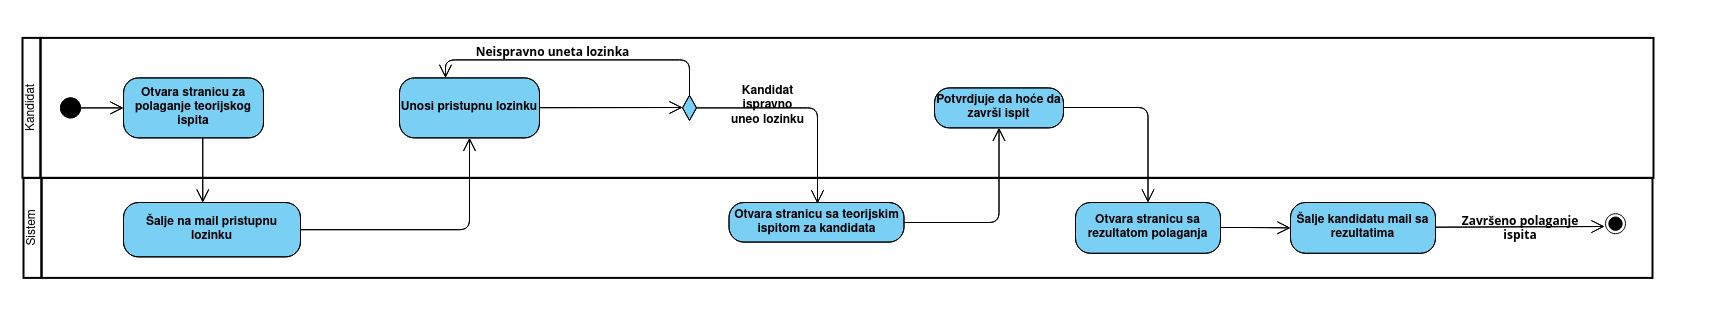
\includegraphics[width=140mm, height=70mm]{Diagrams/polaganje teorijskog ispita.png}
  \end{center}
  \caption {Dijagram aktivnosti - polaganje teorijskog ispita}
  \label{activity_polaganje_teorije}

\end{figure}
